\documentclass{IEEEcsmag}

\usepackage[colorlinks,urlcolor=blue,linkcolor=blue,citecolor=blue]{hyperref}

\usepackage{upmath}

\jvol{XX}
\jnum{XX}
\paper{8}
\jmonth{March/April}
\jname{Computing in Science \& Engineering}
\pubyear{2021}
\newtheorem{theorem}{Theorem}
\newtheorem{lemma}{Lemma}

\setcounter{secnumdepth}{0}

\begin{document}

\sptitle{Jupyter in Computational Science}
\editor{Editor: Thomas Kluyver, thomas.kluyver@xfel.eu}

\title{SlicerJupyter: a 3D Slicer kernel for interactive publications}

\author{Jean-Christophe Fillion-Robin}
\affil{Kitware, Inc}

\author{Andras Lasso}
\affil{{L}aboratory for Percutaneous Surgery at Queen’s University}

\author{Isaiah Norton}
\affil{TileDB, Inc}

\author{Steve Pieper}
\affil{Isomics, Inc}

\author{Sylvain Corlay}
\affil{QuantStack}

\author{Martin Renou}
\affil{QuantStack}

\author{Johan Mabille}
\affil{QuantStack}

\author{Matt McCormick}
\affil{Kitware, Inc}

\author{Mike Grauer}
\affil{Kitware, Inc}

\author{Mike Sarahan}
\affil{RStudio, PBC}

\markboth{Jupyter in Computational Science}{Paper title}

\begin{abstract}
The Jupyter ecosystem is a powerful platform for exploratory computational science, and now it can connect with some of the deep and rich domain-specific desktop applications that have decades of feature development already invested in them. With the integration of 3D Slicer and Jupyter through the xeus-python’s interpreter, we demonstrate how a Qt-based graphical desktop application can be used through a Jupyter notebook with 3D visualization provided by Visualization Toolkit (VTK) and image processing provided by the Insight Toolkit (ITK). This approach is available on the SlicerJupyter GitHub repository and could be extended to other applications that embed Python, such as Blender, FreeCAD, or ParaView.
\end{abstract}

\maketitle


\chapterinitial{The integration of xeus-python}, a python kernel based on xeus, a lightweight C++ based implementation of the Jupyter protocol with few dependencies, is beneficial both for the Jupyter ecosystem and desktop applications. Features that have been developed for decades for desktop applications become readily available for Jupyter users without learning a new working environment or redeveloping features. For a desktop application, the Jupyter notebook can serve as a way to create reproducible data processing workflows, scientific publications, and maintainable tutorials without requiring local software installation. From Jupyter, you can now quickly create simple medical imaging applications with extremely rich interactivity from 3D Slicer. The sections below discuss the features available and the history of the project.

\section{Powerful Medical Imaging Capabilities Available Through Jupyter}

3D Slicer (or Slicer for short) is a C++ desktop application that uses Qt, ITK, and VTK libraries for visualization and medical image analysis. Slicer’s embedded Python interpreter makes all of its features accessible with the Python programming language. Slicer has a simple built-in console to run Python commands interactively and can run Python scripts from files, but these provide a different developer experience that can be augmented by  cell-based interactive notebooks, which have become popular among data scientists and researchers in recent years.

\begin{figure}
\centerline{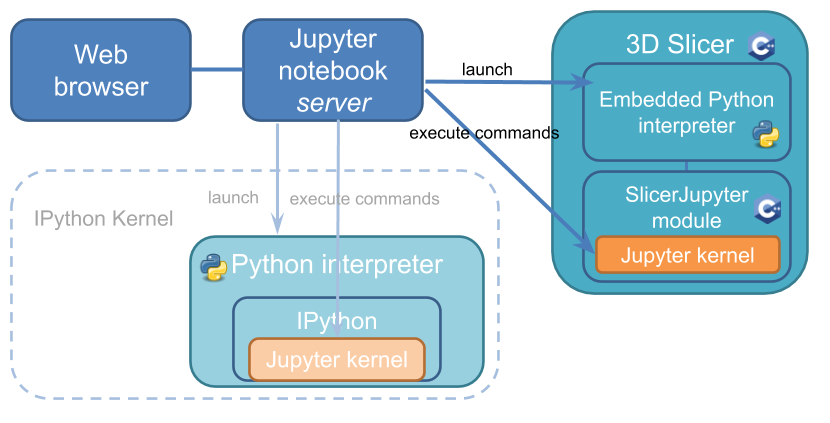
\includegraphics[width=18.5pc]{figure1_kernel_integration.png}}
\caption{Slicer Jupyter kernel runs within the Qt-based application process and communicates with the Jupyter server notebook. This integration allows python commands to be executed from both the Jupyter notebook and from the embedded python interpreter.}
\end{figure}

By integrating the xeus-python kernel, we can use a Slicer process as a Jupyter kernel ({\bf Figure 1}). Xeus-python leverages the xeus C++ implementation of the Jupyter kernel protocol. Xeus-python is an alternative to ipykernel that can be used with a vanilla CPython interpreter to allow interfacing to standard CPython Jupyter widgets like itkwidgets. But it can also be coupled with custom interpreters and GUI event loops, like the Slicer interpreter and its Qt event loop. This allows you to represent a complete scene in Medical Reality Markup Language, MRML, Slicer’s internal data structure. The kernel exposes the full medical imaging API and representation of your data in a meaningful way for Python developers, allowing access through standard Python ecosystem formats such as pandas dataframes and NumPy arrays in the Notebook.

\section{Interactivity Levels}

Jupyter interactive widgets (sliders, buttons, etc.) can be used to control Slicer, modify data, or adjust processing and visualization parameters. Interactivity can be implemented at different levels.

\subsection{Level 1}

Standard Jupyter widgets display application -specific objects by automatic conversion of application-specific data objects to standard Python objects. For example, Slicer markup fiducial lists are displayed as a nicely formatted table ({\bf Figure 2}). and model nodes are rendered as 3D objects ({\bf Figure 3}).

\begin{figure}
\centerline{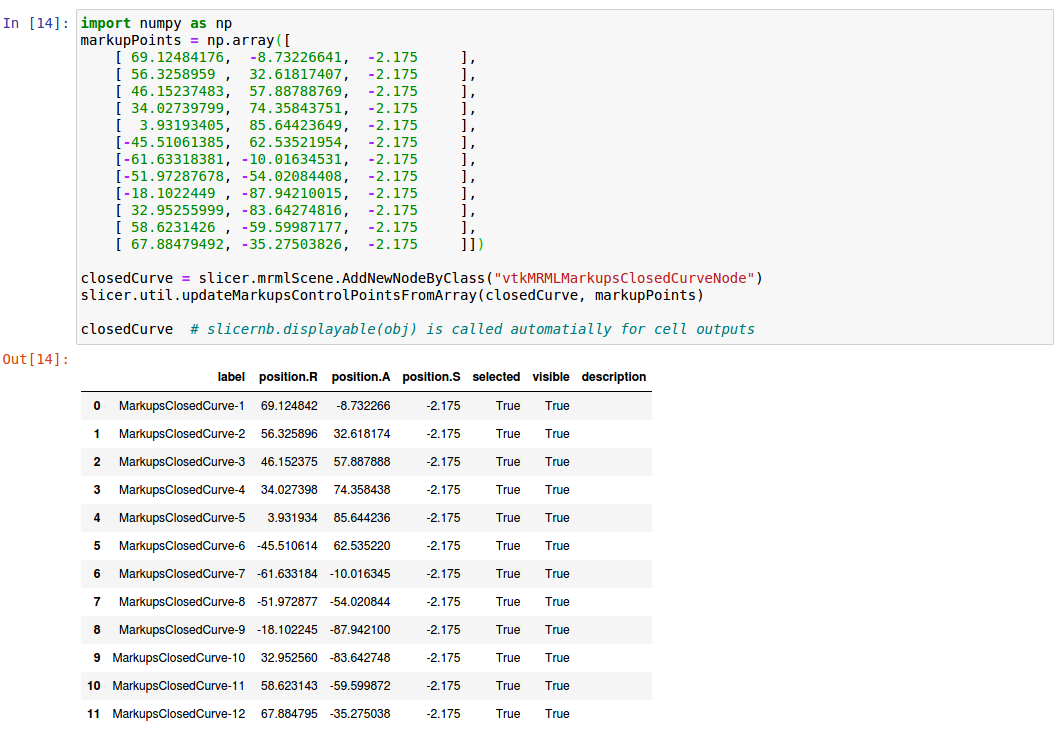
\includegraphics[width=18.5pc]{figure2_markups.png}}
\caption{Slicer markup fiducial lists  automatically rendered as a table.}
\end{figure}

\begin{figure}
\centerline{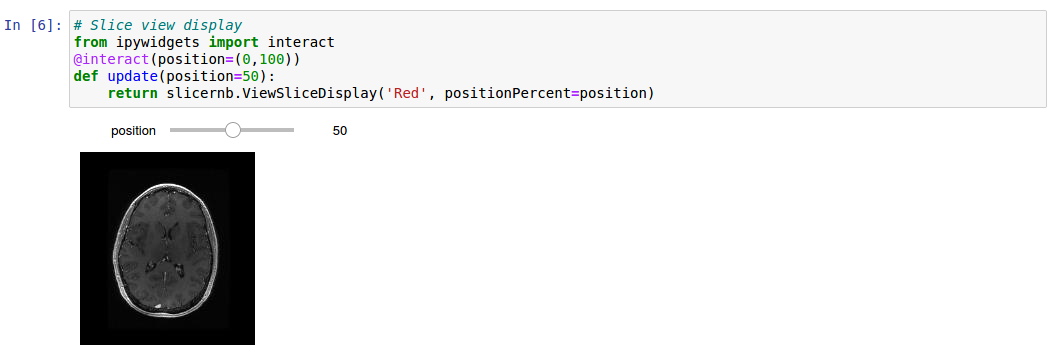
\includegraphics[width=18.5pc]{figure3_model.png}}
\caption{Slicer model rendered as 3D object.}
\end{figure}

\subsection{Level 2}

Static image widgets display content that the desktop application renders. These widgets can be made interactive by modifying data and rendering parameters using additional standard widgets. This makes rich visualization capabilities — sophisticated rendering of various data types, rendering of very large data sets, etc. directly available in Jupyter ({\bf Figure 4}).

\begin{figure}
\centerline{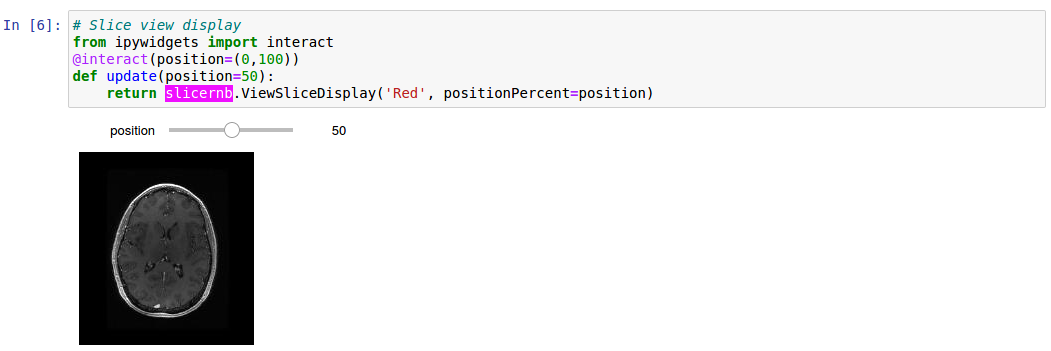
\includegraphics[width=18.5pc]{figure4_slider_update.png}}
\caption{Jupyter slider widget allowing to interactively update the offset along the  axial axis of a MR dataset.}
\end{figure}

\subsection{Level 3}

Dynamic viewer widgets display 2D and 3D views rendered by the desktop application. Mouse and keyboard events are forwarded to the desktop application that allows zooming/rotating views, and to utilize all 3D interactions implemented in the desktop such as placing annotations, making measurements, or segmenting images the same way as if it was done on the desktop application’s screen ({\bf Figure 5}). This is implemented in the Slicer Jupyter kernel using ipycanvas and ipyevents packages.

\begin{figure}
\centerline{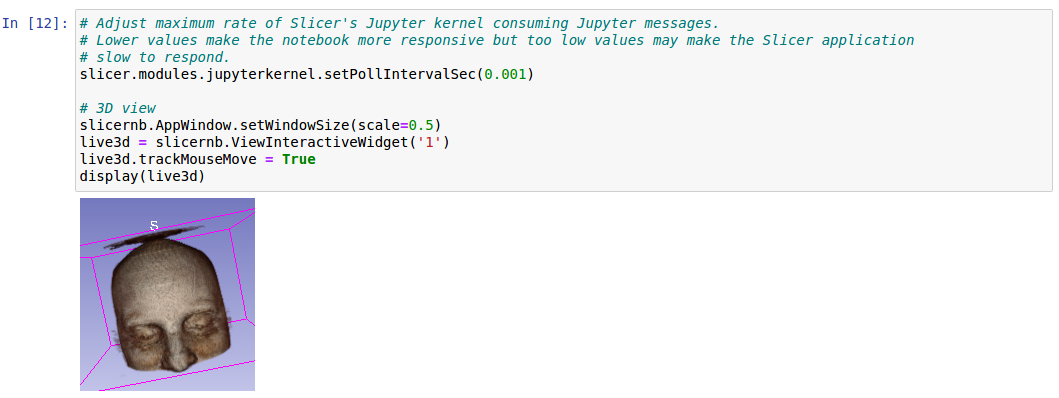
\includegraphics[width=18.5pc]{figure5_interactive_3d.png}}
\caption{Interactive view representing a volume rendering of a MR dataset.}
\end{figure}

\subsection{Level 4}

Full desktop graphical user interface integration allows users to see parts of the application window rendered in notebook cells, including standard desktop widgets (sliders, menus, etc.). It is implemented using noVNC and TigerVNC in Slicer Jupyter. This is particularly useful when the application runs on a remote server.

These interactive tools allow developers to implement complete data processing workflows in a notebook, even if certain steps require manual user inputs such as segmenting 3D regions or setting seed points.


\section{Online Availability using Binder}

Since Jupyter notebooks can be used from any web browser, it can essentially turn any desktop application into a web application. By setting up a remote Jupyter server, users do not have to install anything on their computers. We have set up a demonstration of this using Binder (\url{www.mybinder.org}) that anybody can try at \url{https://mybinder.org/v2/gh/Slicer/SlicerNotebooks/master}.

The docker image that installs and configures Slicer and all dependencies (ipycanvas, ipyevents, VNC, etc.) is available at \url{https://github.com/Slicer/SlicerDocker/tree/master/slicer-notebook}.

For deployment to non-technical users, applications can be deployed using Voilà (\url{https://voila.readthedocs.io/}), which only shows relevant content and interactive widgets, so the notebook looks like a simple dynamic web page.

The current implementation is already stable and offers a wide range of features, but there is still room for design and performance improvements. For example, we could not implement fully automatic conversion of application-specific data objects to displayable Python objects (due to complex implementation of display hooks); xeus-python debugger’s threading model needs to be improved to allow using it without locking the application’s main thread; and the dynamic viewer widget’s performance (level 3 interaction) could be optimized to achieve higher refresh rates.

\section{History of 3D Slicer and this integration}

Built over two decades with support from the NIH and a worldwide open source developer community, 3D Slicer is a multi-platform desktop application for analysis, integration, and visualization of medical images. Slicer is used by researchers globally for basic and applied research in a wide range of topics. The 3D Slicer Community includes physician-scientists with disease-specific knowledge of clinical challenges, computer scientists and physicists who develop novel algorithms, imaging informatics researchers, software engineers with the ability to understand clinical problems and create reliable tools, and application engineers with the multidisciplinary skills to deploy these tools in a range of cancer research settings. Originally developed at MIT and developed by collaborating organizations working with Brigham and Women's Hospital, Slicer is maintained by Kitware, Inc., and has an active international open source software community. Slicer is used in hospitals and by researchers, with more than 10k academic citations and more than 150k downloads in the last year alone (2019/10 - 2020/10).

Slicer can be used for image processing workflows on 2D, 3D, and 4D images. What makes Slicer so useful is its huge set of community contributed modules that extend its functionality, as well as its ability to read DICOM and a wide array of exotic file formats.

Slicer has been scriptable in Python for well over a decade, but a robust SlicerJupyter extension is born from significant development effort by the community. The idea for this integration dates back to SciPy in 2014, when Jean-Christophe Fillion-Robin of Kitware organized a sprint intended to integrate Slicer and an IPython notebook, motivated by the dream of creating interactive and fun tutorials for Slicer. Mike Sarahan and Jean-Christophe created this proof of concept \url{https://github.com/commontk/QEmbedIPython#qt-embed-ipython}, but it was far from usable. In 2015 Matt McCormick of Kitware, created the SlicerDocker repository to support headless builds and rendering in a Docker image. Then in June 2018, while attending the Slicer Project Week, Andras Lasso (Queen’s University) and Jean-Christophe learned about Xeus, a C++ implementation of the Jupyter kernel protocol developed by QuantStack that would help streamline the integration of Slicer with Jupyter. To support this effort, Andras and Jean-Christophe created the Slicer/SlicerJupyter GitHub repository. They also contributed changes to Xeus to support this new integration paradigm where the event loop of the kernel is driven by a Qt-based Desktop application (see here). Building on this foundation, Isaiah Norton, then working at Brigham and Women’s Hospital, contributed additional improvements like a better auto-completion using jedi (see \url{https://github.com/Slicer/SlicerJupyter/pull/12}) as well as integration with Binder. More recently, Jean-Christophe and Sylvain Corlay (QuantStack) met after the 28th Slicer project week while attending SciPy 2018 in Austin (see \url{https://projectweek.na-mic.org/PW28_2018_GranCanaria/Projects/SlicerJupyter/}). Following the creation of a new project called xeus-python (started by Martin Renou at QuantStack), we took the integration of Jupyter and Slicer to the next level by adding support for improved interactive use and MRML data node visualization directly in the notebook.


\section{CONCLUSION}

The integration of Qt-based applications with the Jupyter ecosystem provides a path for leveraging and extending existing tools instead of completely redeveloping something similar in python and for capitalizing on established user and developer communities. It enables the desktop application to remain modern and relevant by running in the cloud via a web browser using a powerful development environment, not just a basic python terminal. It also provides users with a way to share their own workflows. Similarly, the Jupyter ecosystem wins advanced and relevant research features. 

\section{ACKNOWLEDGMENT}

This work was supported in part by NIH grant P41 EB015902.

% \begin{thebibliography}{1}
%
% \end{thebibliography}

\begin{IEEEbiography}{Jean-Christophe Filion-Robin}{\,} is an open-source enthusiast, original author of the SlicerJupyter extension and a principal engineer at Kitware, Inc. where he leads the development of 3D Slicer-based commercial applications. J-Christophe also maintains scikit-build, an improved build system generator for CPython C/C++/Fortran/Cython extensions.
\end{IEEEbiography}

\begin{IEEEbiography}{Andras Lasso.}{\,} is a prolific contributor to 3D Slicer and the original author of the SlicerJupyter extension, Senior Research Engineer and Associate Director of the Laboratory for Percutaneous Surgery at Queen’s University.
\end{IEEEbiography}

\begin{IEEEbiography}{Isaiah Norton}{\,} is a Senior Software Developer at TileDB, Inc. with experience in digital pathology and image-guided surgical navigation.
\end{IEEEbiography}

\begin{IEEEbiography}{Steve Pieper}{\,} is a Chief Architect and active developer of the 3D Slicer application for the last two  decades. He is CEO of Isomics, Inc, where he uses a range of software technologies to perform medical imaging research with leading universities and companies.
\end{IEEEbiography}

\begin{IEEEbiography}{Sylvain Corlay}{\,} is the founder and CEO of QuantStack, and a core Jupyter developer. He co-authored xeus and xeus-python.
\end{IEEEbiography}

\begin{IEEEbiography}{Martin Renou}{\,} is a scientific software developer at QuantStack. He is the original author of xeus-python, the xeus-based Python kernel, and contributed to the new concurrency model used for the debugger.
\end{IEEEbiography}

\begin{IEEEbiography}{Johan Mabille}{\,} is a scientific software developer at QuantStack. He co-authored xeus and xeus-python, developed the new concurrency model for the debugger in both xeus and xeus-python. He also specializes in high-performance computing in C++. 
\end{IEEEbiography}

\begin{IEEEbiography}{Matt McCormick}{\,} is an open source, medical imaging researcher at Kitware, Inc. Matt is an active, contributing member of scientific open source software efforts, such as the Insight Toolkit (ITK) and scientific Python (SciPy) communities, and maintains the Jupyter 3D widget, itkwidgets.
\end{IEEEbiography}

\begin{IEEEbiography}{Mike Grauer}{\,} is a technical leader on the Data and Analytics team at Kitware. He specializes in building scalable server-side processing frameworks that enable scientific workflows over web platforms.
\end{IEEEbiography}

\begin{IEEEbiography}{Mike Sarahan}{\,} is a software engineer at RStudio, PBC working on bringing language ecosystems together. He is passionate about making software work for data scientists in ways that are easy to maintain and improve.
\end{IEEEbiography}

\end{document}

